\section{Implementation}\label{sec:implementation}
Following the theoretical description of the used models, now we present our practical approach. This section is split into the data preparation, explaining our procedure and explicit implementations and lastly, the evaluation of our findings.

\subsection{Data Preparation}
To extract topics or corresponding arguments, we first need data. In this case we use a data-set from \href{https://kaggle.com}{Kaggle} that provides us with the manifestos of all the big parties (CDU, Grüne, SPD, FDP, AfD and Linke) competing in the 2021 German federal election. The data-set is available \href{https://www.kaggle.com/sibelius5/party-platforms-for-the-german-federal-election-21}{on Kaggle}\footnote{\url{https://www.kaggle.com/sibelius5/party-platforms-for-the-german-federal-election-21}}.


The first step in preparing our data was preprocessing. We selected to approach this task in two different ways to see which approach works better. For all our general language processing, we used \href{https://spacy.io/}{spaCy}\footnote{\url{https://spacy.io/}} with the pre-trained \texttt{de\_core\_news\_md} model provided by spaCy \footnote{\url{https://spacy.io/models/de\#de_core_news_md}}.

Firstly, we chose to use a rather explicit approach, tokenizing and lemmatizing our party manifestos with spaCy and then manually selecting what words or word types to filter out. We filtered out stop words, as is common practice, however, also all numbers, URLs, emails, currencies, party names and tokens with certain part-of-speech (POS) tags (verbs in third person singular, adpositions, pronouns and auxiliary words). After filtering all of this, we gathered simple statistics on our words, like what words were used most frequently. This was done to gain a better overview and just get started with text analytics tools in general.

As an example, Figure \ref{fig:spd_stats} shows the word frequencies for the SPD.
 
\begin{figure}[h]
    \centering
    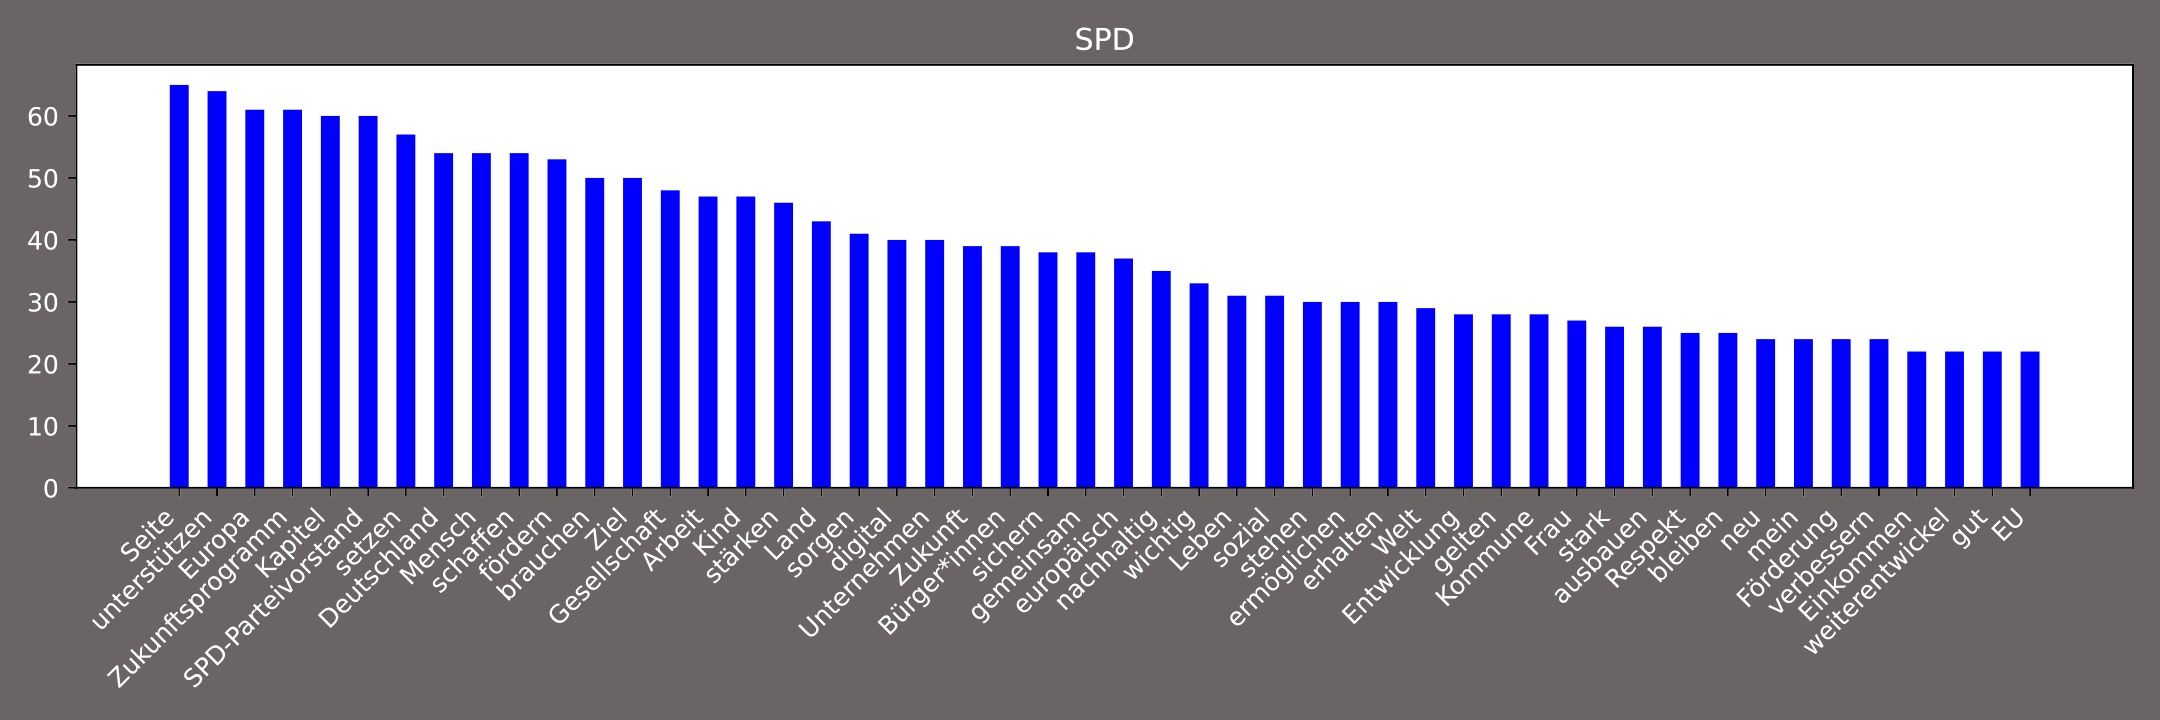
\includegraphics[width=\linewidth]{resources/graph_SPD.png}
    \caption{Word frequencies for the 50 most used words by the SPD in their 2021 federal election manifesto. A larger version can be found in the appendix, Figure \ref{fig:spd_stats_large}.}
    \label{fig:spd_stats}
\end{figure}

In our second approach, we used the \textit{simple\_preprocess} method from gensim which automatically preprocesses data. \textit{simple\_preprocess} lowercases all words and tokenizes the data. Subsequently, we removed stopwords in an extra step, using stopwords from spaCy and nltk. Both spaCy and nltk were used, as some stop words in the spacy corpus were not included in the nltk corpus and vice versa. In total the combined stopword list from spacy and nltk was comprised of 567 words. This extensive list of general stop words was extended manually, to a total size of 696 words. This addition was necessary to not affect our data negatively, as some phrases or words are used in political text and especially manifestos often, but do not usually count as stopwords (e.g. \glqq deutsch\grqq{} as in German or the respective party names). The need for additional stopwords can also be observed in Figure \ref{fig:spd_stats}, where \glqq Seite\grqq{} as in page is the most common word. Another specific word that needed to be amended was the gendered form of words with \glqq\texttt{*innen}\grqq{}, for example \glqq\texttt{Bürger*innen}\grqq{} would be transformed into \glqq\texttt{Bürger}\grqq{}. This change was necessary, as the model would remove the separating star-symbol but treat \glqq\texttt{innen}\grqq{} as a separat word. As a result, \glqq\texttt{innen}\grqq{} would often be among the most frequent word in manifestos that used this style. The left over words were then used to create bi- and trigrams for later use. In addition, the words were lemmatized and all words with POS-tags that were not nouns, verbs, adjectives and adverbs were filtered out. This procedure showed more promising results, so this now heavily processed manifesto text was used in the following steps for topic modelling.

Finally, we manually edited the formatting of party manifestos, as some manifestos did not have clear breaks between paragraphs or graphic formatting dividing a single paragraph in two separate parts. Additionally, all headlines were removed as these would be treated as parts of sentences, due to missing punctuation.

\subsection{Procedure}
In this section, we discuss our different approaches we used in our application. First, we discuss our models used for topic modelling, then how we summarized our texts and finally, our web interface.
\subsubsection{LDA for topic modeling}
We used the \href{https://radimrehurek.com/gensim/index.html}{gensim} framework \cite{rehurek_lrec} for our LDA model. Gensim works by statistically extracting patterns in the given text and linking similarities between documents thus generalizing common topics. % work out gensim better

As we only have one manifesto per Party, we split the manifesto in paragraphs and treat the paragraphs as single documents. We did this, with the premise that every paragraph in a manifesto only focuses on one general topic and thus a good estimation of the topic can be extracted for each paragraph.
For the actual LDA model we used the pre-trained model provided by gensim. The model is given a integer id representation of a each word (id2word) and with these ids a bag-of-words is created and used as our corpus. The LDA model then runs for a specified number of iterations, extracting a number of topics. We settled on 10 topics as this is recommended in literature \cite{gan2021selection} and all manifestos should at least cover 10 separate topics. Through trial and error and analyzing our results we later found five to seven topics to be optimal. We use the (\textit{pyLDAvis}) library which visualizes our topics, showing simple relations between topics and which words are grouped in one topic. As measurements for how accurate and well the model performed, we measured the perplexity and coherence. The specific results and more detailed description will follow in Section \ref{sec:lda_results}. 

As we wanted to have other data to compare our results to, we ran the same process with other models. The models we settled on were LSI and HDP. Similar to the LDA model we measured the coherence of the results. The comparison of LDA, LSI and HDP will also follow in Section \ref{sec:lda_results}. 

% gensim besser herausarbeiten
% LSI und HDP besser beschreiben


\subsubsection{HDP}
At a later point, we tested an other implementation of the HDP model by using the \textit{tomotopy} \cite{bab2min_2021_4999089} framework. This framework is based on the principles of \citet{teh2004sharing} and \citet{newman2009distributed}. With inferred topic and word distributions, the Collapsed Gibbs Sampling (CGS) supports the \textit{tomotopy} framework. Dependening on the number of documents, CGS improves the computation time. When a new topic is considered, every word in a random order will be determined and processed to open up new topics dependent on the probability of an assignment to the current topic. For more details about CGS processes and its optimization possibility look in \citet{subeno2018optimisation}. On this basis, tomotopy can make use of multicore CPUs including a SIMD (Single Instruction, Multiple Data) instruction set for faster iterations \citet{bab2min_2021_4999089}. Here the aim was creating a model to filter party manifesto and receive topics by the uncertainty in their number which is a property of the HDP model. One party manifesto was load as an \textit{Iterable String} for integrating the pretrained model of the HDP by setting it on the number of cores of the system with parameter 0. After that the \textit{burn\_in} iterations for optimization were called with a value of 500.
%Outcomes docs=1(FDP), Vocab=758,TotalWords=8385
Then the word log likelihood was set over a word range of 5000 with a step of 50 and trained with 50 iterations of Gibbs-sampling.
% HDP captures the uncertainty in the number of topics
Whole training process oriented on the model previously mentioned in Section 4 with a minimum collection frequency of documents of 5 and of words of 0. Here the initial parameter of FDPs party manifesto were the number of topics is k=10, the concentration coefficient of DP for document-table $\alpha$=0.1, the hyper-parameter of Dirichlet distribution for topic-word $\eta$=0.01 and the concentration parameter of DP for table-topic $\gamma$=1.0. The first instantiated random seed word value was 99999. After training process the concentration coefficients changed to $\alpha$=6.6722, $\gamma$=66.12 and the Dirichlet Prior on the per-topic word distribution stayed at an value of $\eta$=0.01. Overall generated outcome were 46 topics as well as tables.

\subsubsection{Topic classification on BERT embedding}
% Motivation: Wir haben keine ausgewertet daten -> unsupervised (evtl weak supervised)
% preprocessing -> aufteilen in sections (Annahme: eine sektion nur ein primäres thema)
% sections durch BERT in embedings vektoren um kontext zu schaffen
% CLuster aus LDA -> Themen mit passenden tokens
% ebenfalss in BERT
% Cosine-simularity berechenen und entsprechend zuordnen  as stated by https://dl.acm.org/doi/abs/10.1145/3366423.3380278
Since there is unfortunately no possibility to classify the topics on the basis of completely evaluated data sets for our topic, we have to work only on the basis of the party programs. The idea which we pursue for this, must first of all divide the text into meaningful parts, whereby we make the reasonable assumption that a paragraph in the text primarily revolves around a certain topic.

Based on the work of \citet{Meng2020}, our approach is the classification based on representative tokens for the respective topics. These representative tokens were chosen based on the results of our work with LDA, which yielded the best results for our data. 
We use a pre-trained BERT tokenizer and model to determine the embedding for both the representative tokens and the paragraphs to determine the proximity between the paragraphs and the topics. This model by the \citet{bert-base-german-cased}  is a German BERT implementation that was trained on 2,350,234,427 tokens gathered from a variety of data sets, including a recent Wikipedia dump and News Crawl.

A novelty of our approach is that here, we use word embedding and not only the bag-of-words model. We do not model the individual text with tokens, but instead use this concept of embedding to capture the semantics and structure of our text documents. This significantly improves the topic model and allows it to predict the topics of sections much better than just using a simple bag-of-words model.

We calculate the pairwise Cosine-Similarity in the word vector space based on these vectors to determine the topic that best reflects the paragraph. Each paragraph must be assigned a topic in this manner. For convenience reasons, we use integers as topic ids and just select the closest topic that is most relevant for our paragraph.

\subsubsection{Summary of topics}\label{sec:summary}
As our goal is to show the user a concise overview of topics discussed in the party manifestos, the simple connection of topics to sections is not sufficient. So, for each topic used in our classification, we concatenate every corresponding section gaining a combined text containing all paragraphs classified with a specific topic. This, however, still does not simplify the manifestos and at best orders the sequence of topics. Our next step was then to individually summarize all texts we created in the previous step.
An important requirement for the summary we set ourselves was the need for an extractive summary, meaning sentences in the summary can only be taken verbatim from the original text. We committed ourselves to this obligation, as we did not want to alter the statements given by the party in any way, shape or form, to guarantee reproducible and traceable results.

However, it proved very difficult to find a good model or library to summarize German texts in an extractive manner. Among others, we tested summarizing texts with a few models on huggingface, both German and English models, but did not achieve satisfying results.
After some searching we found \textit{sumy} \footnote{\url{https://github.com/miso-belica/sumy}}, a lightweight library for summarizing texts in various languages, including German. When testing \textit{sumy} with sample texts it worked a lot better than any previous attempts, so in the end we settled on \textit{sumy}. \textit{sumy} incorporates a built-in parser for plain text, files as well as HTML pages. Besides parsers \textit{sumy} offers several types of summarization methods, which can be found on GitHub \footnote{\url{https://github.com/miso-belica/sumy/blob/main/docs/summarizators.md}}. We use LSA (Latent Semantic Analysis) as it is "the most advanced method" and generally yields good results.

\subsection{Results}
In this section we present the results of our previously discussed models. First, the LDA topic modeling results and second the topic classification with BERT embeddings.
\subsubsection{LDA for topic modeling}\label{sec:lda_results}
% fdp pyldavis
% LDA, LSI, HDP vergleich 
% Grafiken einbinden
% resulate aus grafiken \cite{mimno2011optimizing}

The topic clustering with LDA was the first result we obtained during our project.
As can be seen in Figure ~\ref{fig:lda_cluster} with the example of the FDP, it is possible to use LDA to create clusters that represent the topics of the text. 
However, in our data set, the issue is that the overview of the terms contained in the cluster gives a person a natural understanding of the topic, but there is no clear representative that truly describes the cluster's topic.

\begin{figure}[h]
    \centering
    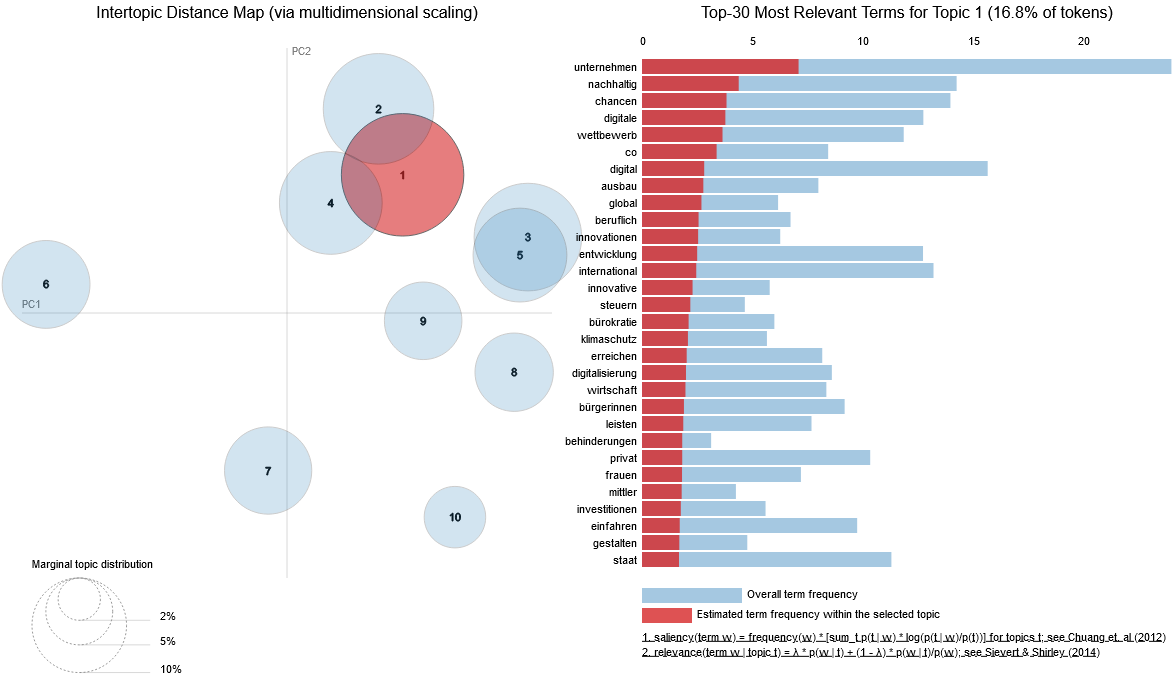
\includegraphics [width=\linewidth]{resources/fdp_cluster.png}
    \caption{LDA visualization at the example of the FDP. A larger version can be found in the appendix, Figure \ref{fig:lda_cluster_large}.}
    \label{fig:lda_cluster}
\end{figure}

Furthermore, it is evident that some topics overlap in a minor or even major way. It can also be seen that the number of topics has a strong influence on the overlap when the number of topics is adjusted, which is why we try to find the best number based on this direct consequence. The coherence score is used to accomplish this. The coherence score indicates how easily the topics can be understood by humans. In our case, the coherence score of a topic may be summarized as follows: If a topic has a high average pairwise similarity with its top $k$ word, it indicates that the topic is very coherent, and can be easily understood by humans. \cite{mimno2011optimizing}
As can be seen in Figure ~\ref{fig:coherence_score}, the coherence score for the first few topics falls\footnote{In gensim u\_mass is always negative and lower values are desirable.} disproportionately, while it continues to fall later, but due to overlaps it is no longer as meaningful. Based on this knowledge, we determine 5 to 7 topics as a good number for party programs. 

In addition, we did the same procedure with LSI and HDP but these methods do not bring us any new insights. However, since they behave the same way as LDA, this check confirms our assumption regarding the number of topics. 


\begin{figure}[h]
    \centering
    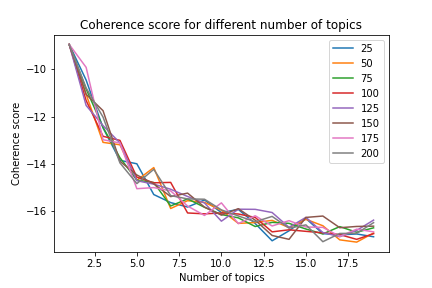
\includegraphics [width=\linewidth]{resources/coherence_score_u_mass_for_CDU.png}
    \caption{U\_MASS coherence score for the CDU. The legend shows the number of epochs for the LDA-Modell}
    \label{fig:coherence_score}
\end{figure}


\subsubsection{Topic classification on BERT embedding}
The output of our BERT implementation is a dictionary with the different parties as the keys and tuples of the most significant sentence-topic pairs as the values. This representation allows a viewer to directly obtain what a party's view on a specific political topic is.

Since the complexity of the self-attention layer inside the transformers is $O(n^2)$ the embedding-conversion is taking quite a while for all the %$\floor{\frac{|T|}{256}}$ 
chunks.

%\subsubsection{Using BERT to get the according text passages}
\subsection{Discussion}
% custom stopwords
In the context of political texts, we have encountered the problem of having a large number of words without meaning, so we decided to introduce context-dependent stopwords.
To bring the texts into a consistent presentation, these contextual stop words include the removal of all gendered language as well as phrases like "we demand..." (wir fordern). No information is lost because these words do not add any expressiveness to the passage's theme. However, we observed that removing them results in much better LDA clusters, with the strongly represented terms now being more representative of the clusters.
In selecting these stopwords, we had to be careful to remove as many as possible in order to get a good result, but also not to be too specific to these texts, so that a generalization still exists and the method could be applied to other party manifestos.

% is topic number realistic
Another finding from our research is an optimal number of 5-7 topics within a text. This finding also makes sense, since within an election the parties have to decide on a reasonable number of issues they want to address. In general, there is a trade off between having fewer, larger topics that are more general and having many, more specific topics.

% results of lda, lsi and hdp
Unfortunately, the LDA, LSI, and HDP clusters we obtain are not as valuable as we had planned for further processing of the party programs. Since it is difficult to select the right appropriate text passages from these clusters, but they assist us in the sense that we can manually evaluate them before applying the knowledge to topic classification on BERT embedding.

% classification
On this foundation, we built a classifier that produced decent results despite the lack of labeled data. There are still some obvious mismatches, but we couldn't get a better outcome by tweaking the parameters. Furthermore, those mismatches are less noticeable after the summerization.


\subsection{Web Interface}
We created a web interface to offer an easy way to interact with our results.
The web interface is a simple \href{https://vuejs.org/}{Vue} \footnote{\url{https://vuejs.org/}} application using \href{https://www.naiveui.com/en-US/os-theme}{Naive UI} \footnote{\url{https://www.naiveui.com/en-US/os-theme}} as a UI framework. The page is available at \href{https://tadl.kalmbach.dev/}{https://tadl.kalmbach.dev/}.

Using the results we gained in the previous sections, we landed on 6 topics, namely environment (Umwelt), economics (Wirtschaft), education (Bildung), society (Gesellschaft), domestic politics (Innenpolitik) and labor and social affairs (Arbeit und Soziales). Then, summaries for every topic were created as described in Section \ref{sec:summary}.

The summaries are presented with no party affiliation to offer a unbiased review. 
Even though, the summaries do not have a clear assignment, summaries can contain phrases which include the party name (e.g. "<Party> promises to ..."). As this is done in several variations and we did not want to introduce bias, we did not remove or hide this type of party affiliation, causing the statements not be entirely anonymous.

Each summary can be rated from one to five stars and after all summaries were rated, a ranking of all parties by stars their respective statements were given is presented.
After completing this for every topic, one can choose to redo the ranking, with the added option of showing directly which summary came from what party. This provides the opportunity to look into specific party manifestos if the summaries were appealing.